\section{Anticommuting Norm Certificates}
\label{sec:norm}

After exact coefficient aggregation, the direct Pauli triangle inequality
$\opnorm{\sum_j c_jP_j}\leq\sum_j|c_j|$ remains sound but unnecessarily loose.
The leading right-generator defect contains many mutually anticommuting
strings.  Their norm is an $\ell_2$, not an $\ell_1$, quantity.

\subsection{Weighted anticommuting groups}

\begin{lemma}[Pairwise-anticommuting Pauli norm]
\label{lem:anticommuting}
Let $P_1,\ldots,P_k$ be Hermitian Pauli operators with $P_i^2=I$ and
$\{P_i,P_j\}=0$ for $i\neq j$.  For real coefficients $c_i$,
\begin{equation}
  \opnorm{\sum_{i=1}^{k}c_iP_i}=\sqrt{\sum_{i=1}^{k}c_i^2}.
  \label{eq:anticommuting-norm}
\end{equation}
\end{lemma}

\begin{proof}
Squaring the sum gives
$\sum_i c_i^2I+\sum_{i<j}c_ic_j(P_iP_j+P_jP_i)$; all cross terms vanish.
Hence every eigenvalue has magnitude $\sqrt{\sum_i c_i^2}$, proving the
operator-norm identity.
\end{proof}

For interval coefficients we replace each $|c_i|$ by its outward rational
upper endpoint and enclose the square root from above.  If
$\mathcal G=\{G_1,\ldots,G_s\}$ is a partition of the Pauli ledger into
pairwise-anticommuting groups, the certified cell bound is
\begin{equation}
 B_{\mathcal G}=\sum_{g=1}^{s}
       \sqrt{\sum_{j\in G_g}|c_j|_\uparrow^2}_{\,\uparrow}.
 \label{eq:grouped-bound}
\end{equation}
Singletons are permitted, so the method is never less sound than termwise
norming and can be applied incrementally.

\subsection{Grouping as a graph certificate}

Construct the anticommutation graph whose vertices are canonical Pauli terms
and whose edges join anticommuting pairs.  A valid group is a clique; a valid
certificate is a vertex-disjoint clique cover.  Finding a minimum-weight cover
is difficult and unnecessary for correctness.  The discovery code uses a
deterministic weighted greedy heuristic that prioritizes large coefficients
and inserts a term only when it anticommutes with every current member.

The verifier does not trust the heuristic.  For every emitted group it checks:
\begin{enumerate}
  \item each referenced Pauli key exists in the coefficient ledger;
  \item every key appears exactly once across the partition;
  \item all distinct pairs satisfy \cref{eq:symplectic-commutation} with
        symplectic parity one;
  \item the squared-weight sum uses the declared coefficient enclosures; and
  \item the rational square-root endpoint squares to at least that sum.
\end{enumerate}
These checks are polynomial in the output size and make optimality irrelevant
to the trusted claim.

\subsection{Leading-defect certificate}

For the degree-four right-generator contribution D4, the concrete ledger has
$75{,}324$ canonical terms.  The emitted partition contains $7{,}576$ groups,
with maximum group size ten.  The resulting per-cell upper bound is
\begin{equation}
  B_{D4}^{\mathrm{group}}=6.472926505087888,
\end{equation}
whereas direct post-aggregation Pauli-$\ell_1$ norming gives
$20.160968407335066$.  The local norm reduction is therefore
$3.114660484942633\times$.  These are certificate statistics, not estimates
from sampled matrices.

\begin{figure}[t]
  \centering
  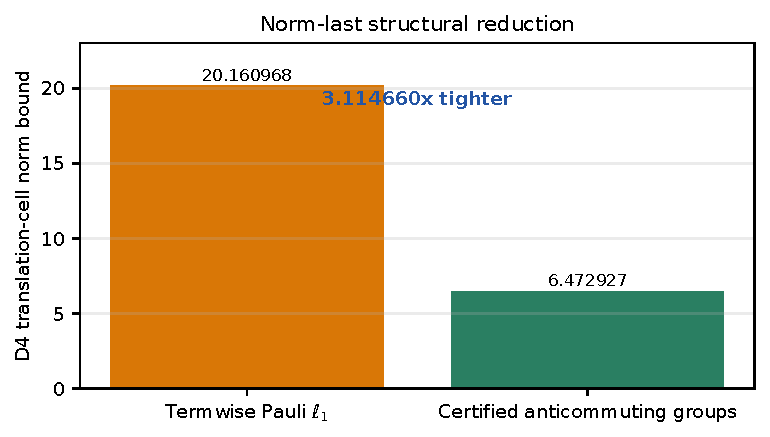
\includegraphics[width=0.68\textwidth]{figures/d4_norm.pdf}
  \caption{Leading D4 cell norm under direct Pauli-$\ell_1$ norming and the
  verified pairwise-anticommuting partition.  Both values are computed after
  exact aggregation; the grouped bar is a rigorous upper bound.}
  \label{fig:d4-norm}
\end{figure}

\subsection{A local Heisenberg identity}

The grouping strategy is reinforced by a small exact algebraic fact.  Let
$h=(XX+YY+ZZ)/4$ on two qubits and let $P$ be a two-qubit Pauli.  Terms of $h$
that commute with $P$ do not contribute to $[h,P]$.  The remaining Pauli
products occur with exactly tracked phases and are pairwise anticommuting for
the local cases used by the certificate.  Consequently the commutator norm is
obtained from a short Euclidean coefficient vector rather than by repeatedly
using $\opnorm{[A,B]}\leq2\opnorm A\opnorm B$.

This lemma is checked exhaustively over the 16 local Paulis.  It supplies an
independent local cross-check on the symplectic engine and explains why the
concrete Heisenberg algebra is substantially smaller than a generic nested
commutator count.  It does not, by itself, prove the global bound; that role is
played by the complete group membership file and finite-step ledger.
